\section{Project Management} \label{Section:Project_Management}
Project management is accomplished through the application and integration of the project management processes of initiating, planning, executing, monitoring and controlling, and closing \cite{PMInstitute:Book}. With any large project, project management is essential to plan the project objectives, scope, deliverables, stakeholders, timeline, and research into appropriate tools that may be used to achieve the project goals. Project management is also necessary to plan for risks and come up with contingency plans. This means that in the case a problem arises, the timeline is not hindered significantly as the problem should already have been considered and a plan to resolve the issue should already exist.

\subsection{Software Development Methodology}
The development of the project followed an agile methodology. This is because the initial project specification, at the time of planning, was not complete and as the project progressed more and more functionality was required which had to be incorporated into the requirements and the system. Another reason that the agile approach was chosen was that as the the project is developed, issues will arise which may not have been accounted for previously. This would not have been possible through a plan driven approach such as waterfall which does not allow the modification of requirements once they've been set out and hence an agile approach is a good way of tackling these issues. 

One fact that must be brought to light is that agile methodologies do not focus on documentation as much as a plan driven approach. Due to documentation being part of the non-functional requirements of this project and a key aspect, a modified version of the agile approach, one where documentation is important, was used. In addition to this rapid prototype development was also employed due to the overlapping of development and testing as this allowed for quick prototype version of components to be created and tested which could then be improved based on the user feedback.


Throughout the development of the project, communication was maintained with stakeholders of the project. This constant stream of communication also resulted in many new features being suggested and implemented and played a key role in the adoption of the agile approach.

\subsection{Project Timeline}
A project timeline was created and represented using a gantt chart in the initial project planning phase, this was included in the project specification and the progress report. This gantt chart is shown in figure \ref{fig:GanttChart}.
 
\begin{figure}[H]
	\centering
	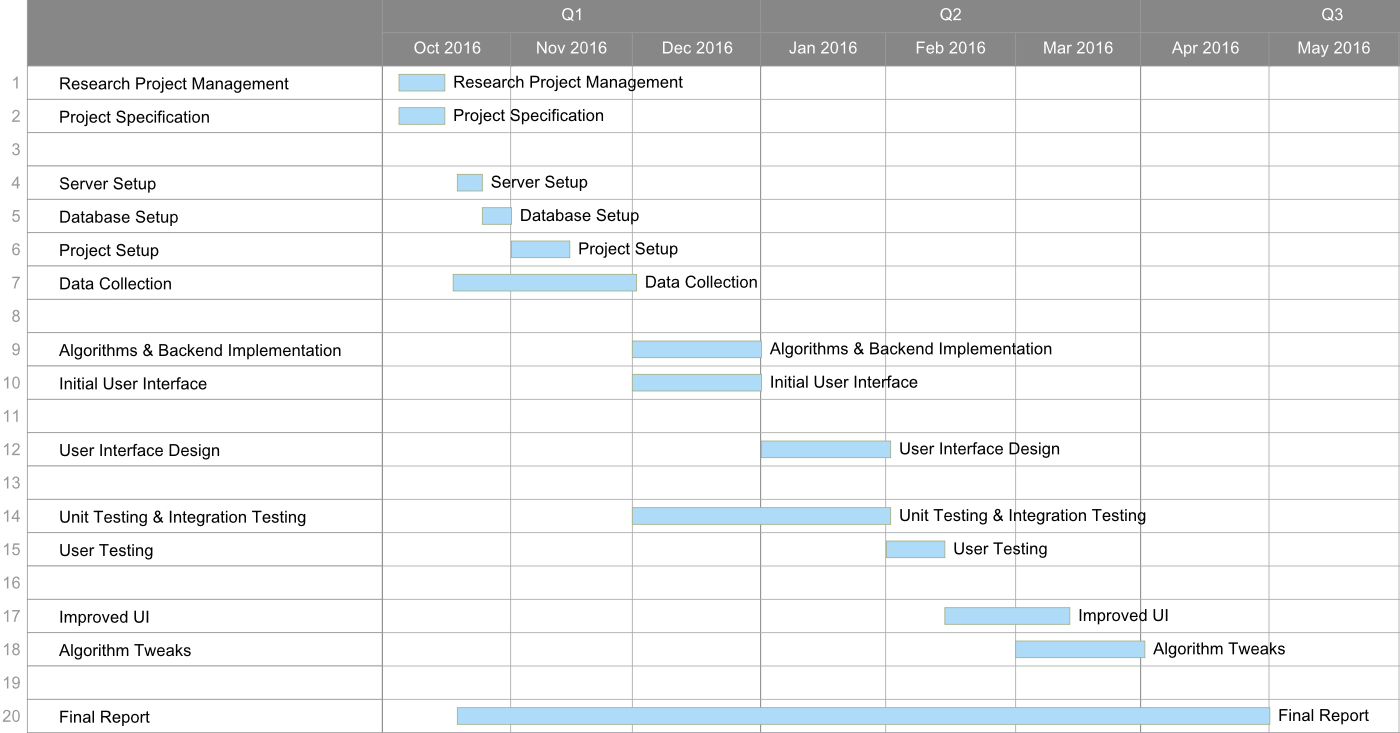
\includegraphics[width=1.0\textwidth]{images/Timeline}
	\caption{Project Timeline Gantt Chart} \label{fig:GanttChart}
\end{figure}

As visible in the gantt chart, many of the tasks are overlapping each other. This is specifically true for development where multiple parts of the system requirement simultaneous development, such as the user interface and the back end functionality associated with the interface. In addition to this, testing and development have been overlapped which allows the user to develop and test the system then go back and improve it based on the results of testing. The overlapping of tasks and development based on feedback highlights the agile approach that was adopted for developing the system as the system is constantly refined until a satisfactory result is produced.

As work was carried out, minor changes were made to the timeline and some tasks were either pushed forward or backward. This is because the requirements were continuously refined resulting in more features being added which were prerequisites for some of the later tasks. Despite the adjusting of the timeline, the development and testing process completed in time and met its final deadline. The remaining time was spent on preparing the presentation for the stakeholder and writing the final report to document the project.

\subsection{Tools and Techniques}
A range of technologies and tools were used for the management and development of the project. This is due to the wide range of support that is available for these tools and technologies which reduces the chance of encountering an issues that the developer cannot solve and saves the developer having to "reinvent the wheel". Using existing frameworks and tools also provides the added benefit that additional features and functionality is implemented by the third-party provider but can be taken advantage of by the developer. The tools employed were used for different tasks, either for developing the project or managing it to ensure a smooth operation, each of which are discussed in further detail below.

\subsubsection{Development}
\begin{figure}[H]
	\centering
	\begin{subfigure}[t]{0.9in}
		\centering
		
\includegraphics[width=0.9in]{images/icons/Laravel}
		\caption{Laravel 5}\label{fig:Laravel}		
	\end{subfigure}
	\quad
	\begin{subfigure}[t]{0.9in}
		\centering
		
\includegraphics[width=0.9in]{images/icons/HTML_5}
		\caption{HTML 5}\label{fig:HTML_5}
	\end{subfigure}
    \quad
	\begin{subfigure}[t]{0.9in}
		\centering
		
\includegraphics[width=0.9in]{images/icons/CSS_3}
		\caption{CSS 3}\label{fig:CSS_3}
	\end{subfigure}
    \quad
	\begin{subfigure}[t]{0.9in}
		\centering
		
\includegraphics[width=0.9in]{images/icons/JavaScript}
		\caption{JavaScript}\label{fig:JavaScript}
	\end{subfigure}
    \quad
	\begin{subfigure}[t]{0.9in}
		\centering
		
\includegraphics[width=0.9in]{images/icons/PHP_7}
		\caption{PHP 7}\label{fig:PHP_7}
	\end{subfigure}
	\quad
	\begin{subfigure}[t]{0.9in}
		\centering
		
\includegraphics[width=0.9in]{images/icons/MySQL}
		\caption{MySQL}\label{fig:MySQL}		
	\end{subfigure}
	\quad
	\begin{subfigure}[t]{0.9in}
		\centering
		
\includegraphics[width=0.9in]{images/icons/jQuery}
		\caption{jQuery}\label{fig:jQuery}
	\end{subfigure}
    \quad
	\begin{subfigure}[t]{0.9in}
		\centering
		
\includegraphics[width=0.9in]{images/icons/Google_Maps}
		\caption{Maps}\label{fig:Google_Maps}
	\end{subfigure}
    \quad
	\begin{subfigure}[t]{0.9in}
		\centering
		
\includegraphics[width=0.9in]{images/icons/Met_Police}
		\caption{Met Police}\label{fig:Met_Police}
	\end{subfigure}
    \quad
	\begin{subfigure}[t]{0.9in}
		\centering
		
\includegraphics[width=0.9in]{images/icons/Apache}
		\caption{Apache}\label{fig:Apache}
	\end{subfigure}
	\caption{Development Tools Employed}\label{fig:DevelopmentTools}
\end{figure}

A wide range of technologies were used for the development of the project, some of which are shown in figure \ref{fig:DevelopmentTools}. Research into each of these technologies along with their advantages and disadvantages is provided in section \ref{Section:Research_Technologies}. Section \ref{Section:Implementation} further discusses some of the core technologies such as Laravel, PHP, MySQL, jQuery and provides reasons for their use \cite{Laravel:Home, PHP:Home, MySQL:Home, jQuery:Home}. In addition to these core technologies, several smaller tools and technologies were also used. The majority of the user interface was developed using HTHML 5, although some of this was generated using the Laravel Blade engine, and styled using Bootstrap or custom Cascading Style Sheets \cite{W3:HTML5, Bootstrap:Home, W3:CSS}. Majority of the backend development was carried out using the popular scripting language PHP but some of this was also automatically generated using syntax provided by the Laravel Blade engine \cite{PHP:Home, Laravel:Blade}. 


The Google Maps and police API were used together to generate a crime map around the users current location which highlights all instances of theft or burglary that were reported to the police in the last year \cite{Google:Maps, Police:API}. In addition to this, the Google Map API was also used to coding and decoding coordinates and addresses that were used to plot locations on the dashboard and stolen items on the search page \cite{Google:GeoCoding}. A MySQL database was used to store the data which could then be queried through SQL, or using the Laravel Query Builder \cite{MySQL:Home, Laravel:QueryBuilder}. Although Laravel provides a lightweight deployment web server, which was used to serve the application on the local development, Apache was used to serve the application on the production server \cite{Laravel:Home, Apache:Home}.


\subsubsection{Management}

\begin{figure}[H]
	\centering
	\begin{subfigure}[t]{0.9in}
		\centering
		\includegraphics[width=0.9in]{images/icons/PHPStorm}
		\caption{PhpStorm}\label{fig:PHPStorm}		
	\end{subfigure}
	\quad
	\begin{subfigure}[t]{0.9in}
		\centering
		
\includegraphics[width=0.9in]{images/icons/Github}
		\caption{Github}\label{fig:Github}
	\end{subfigure}
    \quad
	\begin{subfigure}[t]{0.9in}
		\centering
		
\includegraphics[width=0.9in]{images/icons/DigitalOcean}
		\caption{DigitalOcean}\label{fig:DigitalOcean}
	\end{subfigure}
    \quad
	\begin{subfigure}[t]{0.9in}
		\centering
		
\includegraphics[width=0.9in]{images/icons/Wunderlist}
		\caption{Wunderlist}\label{fig:Wunderlist}
	\end{subfigure}
    \quad
	\begin{subfigure}[t]{0.9in}
		\centering
		
\includegraphics[width=0.9in]{images/icons/Trello}
		\caption{Trello}\label{fig:Trello}
	\end{subfigure}
	\caption{Management Tools Employed}\label{fig:ManagementTools}
\end{figure}

All the code written throughout the development process was done using an IDE provided by JetBrains called PhpStorm \cite{JetBrains:PHPStorm}. PhpStorm provides syntax highlighting, code completion, and numerous other features for all major web development technologies. Optional plugins can be installed provide support for even more technologies, as done for Laravel \cite{JetBrains:PHPStorm}. PhpStorm also provides integrated support for Git which was used to provide version control for all the code written. This allowed files to be added to Git as soon as they were created so they would not be omitted from commits, causing inconsistencies \cite{JetBrains:PHPStorm}. The use of Github allowed code to be backed up online, in case of a hardware failure, so it could be replicated onto another machine easily \cite{Github:Home}. This was particularly useful when deploying the code from the development server to the production server hosted by DigitalOcean\cite{DigitalOcean:Home}. As soon as a feature was fully implemented, it could be pushed up to the Github servers allowing for the changes to be fetched by the production server just by issuing a single command. 

\begin{figure}[H]
	\centering
	
\includegraphics[width=1.0\textwidth]{images/Trello}
	\caption{Trello: Project Work Breakdown Structure} \label{fig:Trello_WBS}
\end{figure}

A number of desktop and web applications were used to keep track of the daily development progress and any remaining work that needed to be completed. Wunderlist was used to keep track of daily tasks that needed to be completed whereas Trello, as shown in figure \ref{fig:Trello_WBS}, was used to keep an overall development log of all the features that were to be implemented \cite{Wunderlist:Home, Trello:Home}. These were strictly for the developer and hence to communicate this progress, emails and face to face meetings were used to update the project supervisor and stakeholders. All the tools discussed are illustrated in figure \ref{fig:ManagementTools}.

\subsection{Risk Management}
When taking on a project, there will always be risks associated with it. Before starting the project, it is important to consider these risks and generate contingency plans to deal with theses ricks, should they arise. As with all project, there were several risk associated with this project due to the nature of the services being offered. Some of these risks are naturally exist for all projects, such as a member of the team falling ill, whereas others are introduced by the reliance on third party services. Sometimes, even the users of the system may present risks which need to be dealt with. The most severe of these risks along with plans to deal with them are discussed below.

\subsubsection{Developer Sickness}
It is likely that throughout the course of this project, over a year, the developer may be faced with illness or another unavoidable crisis which may leave the developer unable to work on the system for a short period of time. In a group project, this could be overcome by always keeping group members in the loop so they could carry on but this is not possible for an individual project. As there is no way to strictly prevent this issue from occurring, the focus should be on minimising the affect in the case that it does occur. With this in mind, a flexible project timeline was created which allowed room for time periods in which development could be paused, tasks could be allowed to overrun, or later tasks could be started early without affecting later tasks or overall project deadline. This can be seen on the timeline where the end of a task overlaps the start of another task. The timeline incorporates this for various reasons, such as certain components taking longer than expected, and the developer falling ill is on of them. Additionally, the use of an agile methodology along with rapid prototyping means that a functional prototype of the system is always available, although it may be limited.

\subsubsection{Hardware Failure}
The machine used to host the local development server is a personal laptop, used on a regular basis for a variety of tasks, making it prone to failure from many different issues. In addition to this, a third party service was being used for hosting the production server on a VPS. This meant the hardware for this was reasonably stable as regular maintenance is carried out and quality assurance is provided by the service provider. As a result, it was only important to consider a hardware failure on the local side. In order to deal with this, two different approaches were adopted. The first approach employed a syncing service known as dropbox which maintained a copy of the code in the cloud, consistent with the development copy. This meant that in the case of a failure, all the code could be restored by downloading a copy from the cloud. The second approach employed a git services knowing as Github which maintained a copy of the code up to the last checkpoint. The two backups together guaranteed that either the code could be completely restored or the last functioning checkpoint could be restored in the case of a system failure. No local copies of the code were kept on backup drives as it was highly unlikely that both cloud services would fail at the same time.

\subsubsection{Data Exposure}
Data security is a key issues that has been repeated many times throughout the project report. An exposure of user data could leave the system and the developer vulnerable to the law so it is important to ensure that in the case that user data is exposed, there is a plan in place to protect the users and the developer. SQL injection is an extremely common means of gaining unauthorised access to the database and there have been many cases of it. It was decided that user credentials will be hashed before being stored in the database, making it almost impossible for anyone to decrypt the data within a reasonable period of time. In order to protect users privacy and their location, any locations they registered would only be approximate to their postcode and street rather than their door number. This is because location data could not be hashed as it has to be retrieved and displayed throughout the system. Finally, the database was protected by a password to prevent unauthorised access to any of the data.

Another piece of data that needs to be protected is any content that is uploaded by the user. Users can navigate to the URL where all the uploaded content is stored and freely browse it. To prevent this from happening, all directories user content have bee made private and protected through rerouting rules using ".htaccess" and PHP. This means that resources can only be viewed if a user has a direct to link, not by simply browsing through the directory structure. Additional security has been added by generating random name for folders and files and then storing these in a database so users cannot simply guess the URL of content. The random paths also make it difficult to identify a user using their resources. 

\subsubsection{Third-Party Services}
The system relies heavily on services provided by third-party APIs, making it vulnerable to failure if these services were to be revoked or updated. The Google Maps API is used throughout the system for a number of features ranging from generating maps and plotting markers to translating coordinates and addresses. Without this service, it would be almost impossible to automatically retrieve the users address from their coordinate or post code. Were these services to be revoked, the user would be able to complete the entire address form by themselves rather than having it filled in by the autocomplete feature which used the Google Maps API. Additionally, where maps are used, alternate visualisation options, such as display the results as a list instead of markers on a map, have been provided so that the user may continue to use the system in the absence of these services. 

Additionally, the system may not function as planned if these services were to be updated. This problem can be overcome by constant maintenance to ensure that the system is kept up to date.

\newpage